%% LyX 2.2.1 created this file.  For more info, see http://www.lyx.org/.
%% Do not edit unless you really know what you are doing.
\documentclass[english]{article}
\usepackage[latin9]{inputenc}
\usepackage{graphicx}
\usepackage{babel}
\begin{document}

\title{Reinforcement Learning Written Assignment - 1}

\author{Akshit Kumar (EE14B127)}

\date{21st January 2017}
\maketitle
\begin{abstract}
This assignment contains the solutions to the first written assignment
of the course Reinforcement Learning. The problems in the assignment
are from the first chapter of the book Reinforcement Learning : An
Introduction by Sutton and Barto.
\end{abstract}
\begin{quote}
\pagebreak{}
\end{quote}

\section*{Exercises}

\subsection*{Exercise 1.1 Self Play}

Suppose, instead of playing against a random opponent, the reinforcement
learning algorithm described above played against itself, with both
sides learning. What do you think would happen in this case? Would
it learn a different policy for selecting moves?

\subsection*{Solution 1.1}

In the case of self play the reinforcement learning agent will learn
to play against itself and eventually the policy will converge to
a minimax strategy. The algorithm makes use of an $\epsilon$-greedy
approach wherein it moves greedily with a probability of $1-\epsilon$
where $\epsilon=0.1$(say). So most of the time the RL agent exploits and
makes a move to enter a state from which its probability of winning
is maximum. A similar strategy is followed by the opponent RL agent
in terms of selection of moves. This in effect converges to a minimax
game strategy where in the minimax algorithm, the \textquotedblleft agent\textquotedblright{}
following the minimax algorithm search through the entire state space
and enters a state from which it can\textquoteright t lose. We can
show empirically that learning through self play leads to a better
policy than by playing against a random opponent using the plot below
:

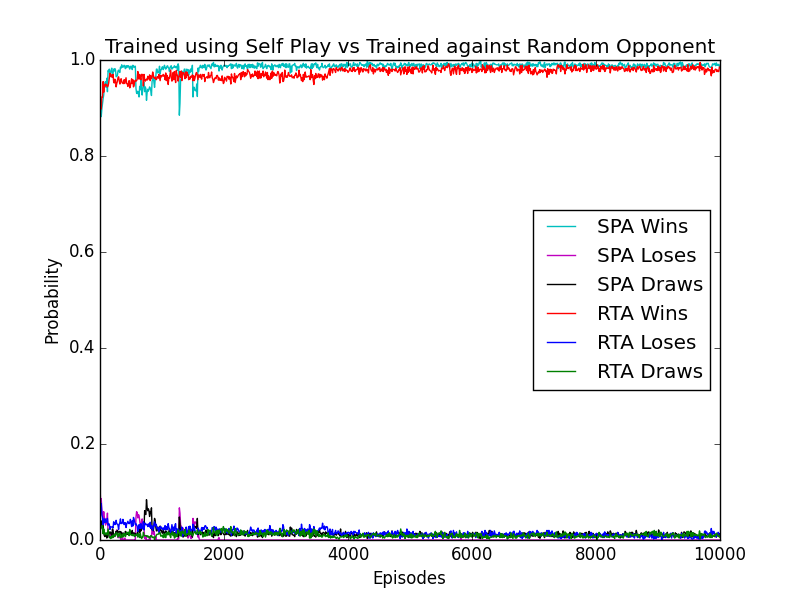
\includegraphics[scale=0.6]{tictactoe-rl/result_selfplay_random}

Here, SPA stands for Self Play Agent which the RL agent trained using
self play that is by playing against itself and RTA stands for Randomly
Trained Agent which the RL agent which is trained against a random
opponent. After certain rounds of training the agent trained respectively
play against a random opponent where they each try to act optimally
ie $\epsilon=0$ during testing. One can clearly see that the policy
learnt using self play is that of minimax as lose probability of agent
trained using self play becomes 0 after a few episodes after which
it either draws or wins and since it is playing against a random opponent
it wins most of the matches. The graph above is for an agent is trained
to learn the strategy for a \emph{player which starts the game}. 

\subsection*{Exercise 1.2 Symmetries}

Many tic-tac-toe positions appear different but are really the same
because of symmetries. How might we amend the learning process described
above to take advantage of this? In what ways would this change improve
the learning process? Now think again. Suppose the opponent did not
take advantage of symmetries. In that case, should we? Is it true,
then, that symmetrically equivalent positions should necessarily have
the same value?

\subsection*{Solution 1.2}

A tic-tac-toe board has 4 axis of symmetries. So if you are in a given
state ie a possible board position, by rotating the tic-tac-toe board
about these axis of symmetries you can reach another state (a possible
board position). The Value Function Based Method employed to learn
an optimal policy for playing tic-tac-toe can be amended by tying
up all the symmetric states as a single state. This can be achieved
by updating the value function of all the ``legal'' symmetric states
of a given state whenever we are updating the value function for that
particular state. This would significantly improve the time taken
to learn the policy as we would operate on a dimensionaly reduced
state space. To illustrate the point, let us say that we are in state
$S_{1}$and have a board position $B_{1}$and the value function for
winning from this state is say 0.85 that is we might have come across
this board position multiple times in the past have gone on to win.
Now consider a symmetric state $S_{2}$with a mirror symmetric board
position $B_{2}$ie the board position is flipped about the horizontal
axis, it might happen that during the learning stage,we might not
have visited this state very often but by winning from state $S_{1}$and
winning from state $S_{2}$should have the same value function asymptotically,
hence by exploiting the symmetries,we can simultaneous update the
value function of all symmetric positions just by knowing the value
function for one board position. This may also lead us to discover
state which we probably might not have discovered by considering all
the states unique.

If the opponent was taking advantage of symmetries, even we should
take advantage of it as this would enable us to learn a better policy
against this type of opponent. If the opponent was not taking advantage
of symmetries, then neither should we because the agent won't learn
by exploiting that states whose symmetrically equivalent states have
been exploited. Hence, symmetrically equivalent positions should not
necessarily have the same value

\subsection*{Exercise 1.3 Greedy Play}

Suppose the reinforcement learning player was greedy, that is, it
always played the move that brought it to the position that it rated
the best. Might it learn to play better, or worse, than a nongreedy
player? What problems might occur?

\subsection*{Solution 1.3}

The RL agent uses an $\epsilon-$greedy algorithm to resolve the ``explore-exploit''
dilemma wherein it makes a ``\emph{greedy move}'' with probability
of $1-\epsilon$ and makes a ``\emph{random move}'' (ie explores)
with a probability of $\epsilon$. By setting $\epsilon=0$ we can
turn the algorithm into a greedy play algorithm wherein the agent
will always ``\emph{exploit}'', in this case the agent will have
an advantage in the initial few games and would win more games compared
to a non-greedy player but over time the greedy player will converge
to a sub-optimal policy and keep on playing that sub-optimal policy
for all the episodes hanceforth as it would not learn any moves which
could possibly have resulted in more wins. After some $n$ number
of games, the non-greedy agent would have learnt about way more actions
and their respective reward signals than the greedy player and can
then exploit the state space way better than the greedy-player. 

Initially the ``regret'' for greedy player will be lower than that
of a non-greedy player as a non greedy-player will make random moves
to explore states with may end in a loss but after a sufficient number
of games, the non-greedy player will converge to the true probabilities
of winning from a certain state whereas the greedy player will just
converge to a sub-optimal policy or may eventually converge to an
optimal policy but after playing infinitely many games hence the ``cummulative
regret'' in the case of greedy player will be more than that of the
one in non-greedy player. This can also be shown empirically using
the figure.

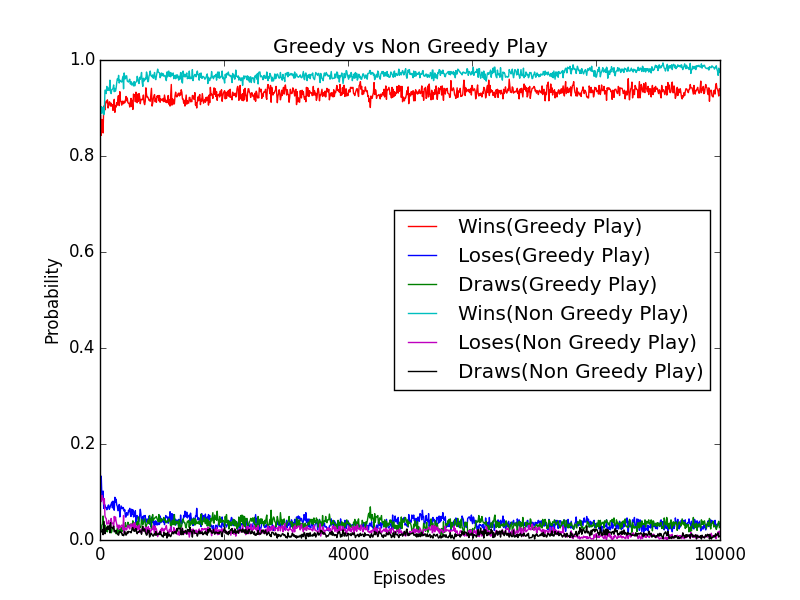
\includegraphics[scale=0.6]{result_epsilon_zero}

The graph above shows the probabilty of wins/loses/draws over 10000
episodes. It can be clearly seen that a non-greedy player($\epsilon=0.1$)
performs better than a greedy player ($\epsilon=0$).

\subsection*{Exercise 1.4 Learning from Exploration}

Suppose learning updates occurred after all moves, including exploratory
moves. If the step-size parameter is appropriately reduced over time
(but not the tendency to explore), then the state values would converge
to a set of probabilities. What are the two sets of probabilities
computed when we do, and when we do not, learn from exploratory moves?
Assuming that we do continue to make exploratory moves, which set
of probabilities might be better to learn? Which would result in more
wins?

\subsection*{Solution 1.4}

If we do not learn from exploratory moves, we would converge to a
set of probabilities which are set of probabilities for an optimal
policy and the strategy would be equivalent to that of playing a minimax
strategy. According to this learnt policy we will be presented with
the best possible move (the one which maximise our chance of winning)
given a particular board position. If we do learn from exploratory
moves, we ``might'' learn a set of incorrect probabilities for a
state. Exploratory moves are more often non-optimal actions for the
given state as it is randomly choosen. The rewards resulted by those
actions will be negative (or positive) though the value obtained after
a series of actions might be positive (or negative). Hence, learning
from exploratory moves might give a wrong probability and feedback
about the action taken. To illustrate this point, let us consider
that we are in state $S_{1}$ and from there we can go the following
states $s_{1}^{*},s_{2},s_{3},.............,s_{n}$ where $s_{1}^{*}$ is
the state we would reach if we choose optimal and that state may result
in a win but since we are exploring we might randomly choose a non
optimal state say $s_{4}$ which results in a lose, now if we learn
from our exploratory move, we would go back and decrease the value
of function of state $S_{1}$ such that it ends up becoming a non-optimal
state and hence we end up penalizing a state for choosing an action
which it ideally would not have chosen and hence we may converge to
a set of incorrect probabilities.

As illustrated above, not learning from exploratory moves will result
in larger number of wins as compared to learning from exploratory
moves because we would be using the optimal policy in the first case.

\subsection*{Exercise 1.5 Other Improvements}

Can you think of other ways to improve the reinforcement learning
player? Can you think of any better way to solve the tic-tac- toe
problem as posed?

\subsection*{Solution 1.5}

Following are some of the ways to improve the reinforcement learning
player and solve the tic-tac-toe problem in a better way:
\begin{itemize}
\item Have a different reward assignment for a state which results in a
loss or a draw. The algorithm described in the book assigns the same
reward to a loss and draw state. Instead of that we can penalise the
agent for entering into a state which results in a loss by assigning
it a negative reward signal. One such possible reward assignment could
be $+1$ for a win, $0$ for a draw and $-1$ for loss. This would enable
us to converge to the optimal policy quicker than using the same reward
for draw and loss.
\item Set up a look up table for certain states. There will exist certain
board positions from which a win/draw/loss is definite respectively.
Therefore we can create a dictionary of such moves so that whenever
the agent enters a state in the dictionary, the action is fixed and
it doesn't choose the move in accordance to the value function. This
will decrease the time it would take to converge to the optimal policy.
Instead of a look up table, we could also increase the value function
of states that result in win and decrease the value function of states
that result in loss drastically so that we are forced to choose a
certain move and forced to not choose a certain move when we are in
state from which we can win or loss respectively.
\item (\emph{Use Minimax Algorithm}) Since the tic-tac-toe is pretty small
and easy, it can be solved recursively and we can do a bruteforce
search through the entire state space and make moves which never put
us in a position from which we can lose.
\item Start with a large value of $\epsilon$ initially and then decrease
it over time. This would result in the agent exploring more initially
and converging to the optimal solution quicker than having a constant
$\epsilon$. As we play more number of games, we will be more confident
of optimal moves as we would have explored more and eventually with
time we can reduce the exploration and only pick optimal moves. One
downside of this method is that initially we would receive a lot of
regret but we will be asymptotically close to the optimal policy quickly.
\end{itemize}

\section*{Appendix}

The plots generated for the results are using a simulation. The code
for the simulation : https://github.com/AkshitKumar/CS6700/blob/master/tictactoe-rl/tictactoe.py
\end{document}
